% Don't modify this section unless you know what you're doing!
\documentclass[letterpaper,12pt]{article}
\usepackage{float}
\usepackage[spanish]{babel}
\selectlanguage{spanish}
\usepackage[utf8]{inputenc}
\usepackage{tabularx} % extra features for tabular environment
\usepackage{amsmath}  % improve math presentation
\usepackage{graphicx, wrapfig, subcaption, setspace, booktabs}
\usepackage{graphicx} % takes care of graphic including machinery

\usepackage[margin=1in,letterpaper]{geometry} % decreases margins
\usepackage{cite} % takes care of citations
\usepackage[final]{hyperref} % adds hyper links inside the generated pdf file
\usepackage{amsmath}
\usepackage{amssymb}
\usepackage{enumerate}
\usepackage{url}
\hypersetup{
	colorlinks=true,       % false: boxed links; true: colored links
	linkcolor=blue,        % color of internal links
	citecolor=blue,        % color of links to bibliography
	filecolor=magenta,     % color of file links
	urlcolor=blue         
}
%++++++++++++++++++++++++++++++++++++++++
\documentclass{article}
\usepackage[utf8]{inputenc}

\title{Actividad 11}
\author{Daniela Olmos Velderrain}
\date{27 de mayo del 2019}

\begin{document}

\maketitle

\section{Introducción}
En esta actividad se analizó de nuevo la ecuación de Duffing, explorando los diversos movimientos que posee este oscilador. Se elaboraron gráficas de posición contra tiempo y su retrato fase, donde se describen distintos estados de este sistema dinámico al modificar una de sus condiciones iniciales.\\\\
Para hablar sobre los resultados obtenidos, se expondrá también una breve introducción a la teoría del Caos, mostrando un poco de su contexto histórico.
           
\section{Desarrollo}
            
\subsection{Marco teórico}
\subsubsection{Teoría del Caos}
\begin{wrapfigure}{l}{0.3\textwidth}
    \centering
    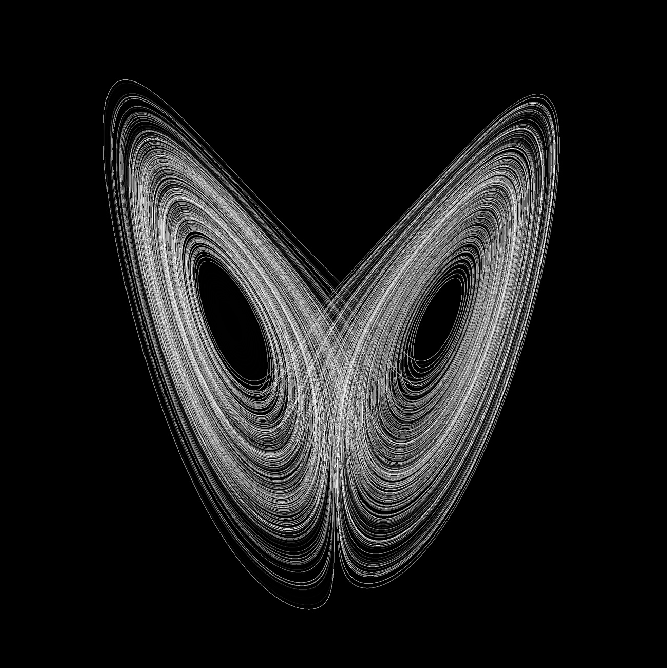
\includegraphics[width=0.3\textwidth]{loo.png}
    \caption{Atractor de Lorenz.}
\end{wrapfigure}


La teoría del caos es una rama de las matemáticas que se centra en el estudio de sistemas dinámicos sumamente sensibles a las condiciones iniciales.  
\\\\
Muchos sistemas naturales exhiben un comportamiento caótico, como el clima, las turbulencias y las finanzas.
En estos sistemas, pequeñas diferencias en las condiciones iniciales llevan a resultados completamente diferentes, haciendo imposible una predicción a largo plazo de su comportamiento.
\\\\
Edward Lorenz fue el primero en reconocer un comportamiento caótico en el modelado de sistemas meteorológicos. Lorenz trabajaba desarrollando modelos climáticos en 1961, utilizando una computadora para realizar sus cálculos. Intentando reproducir una simulación, se dio cuenta de que al introducir condiciones iniciales con diferencias mínimas en su modelo se generaban resultados ampliamente divergentes. 
\\\\
En 1963 Lorenz introdujo un concepto denominado \emph{atractor de Lorenz}. Este es un sistema dinámico determinista tridimensional no lineal obtenido de las ecuaciones simplificadas de rollos de convección producidos en las ecuaciones dínámicas que modelan la atmósfera terrestre. 
\\\\ 
Su forma pudo haber inspirado el nombre del concepto de la teoría del Caos conocido como \emph{efecto mariposa}. Según el efecto mariposa, dadas ciertas condiciones iniciales en un sistema dinamico caótico, cualquier discrepancia mínima entre dos situaciones iniciales dará lugar a nuevas situaciones donde la evolución de cada sistema será completamente distinta, implicando que cualquier perturbación pequeña (como el aleteo de una mariposa) puede generar efectos insólitos a largo. 

\subsubsection{Teoría de las Bifurcaciones}
 En sistemas dinámicos, una bifurcación ocurre cuando una pequeña variación los parámetros de un sistema causa un abrupto cambio "cualitativo" en su comportamiento.\\
 Esta teoría pretende explicar como se modifica el comportamiento de los sistemas en determinadas circunstancias, de manera que en lugar de seguir un comportamiento determinado éste cambia a otro de forma brusca. De esta forma, si el sistema seguía una desarrollo dado, en cierto punto lo modifica por otro que lo dirige hacia un objetivo completamente diferente.\\ 
No importa que la trayectoria que seguía hasta este momento fuese uniforme  y tuviese oscilaciones más o menos regulares, en un punto el sistema modifica de forma radical su dirección, propósito u objetivo. 
    

\subsection{Metodología}
Para esta actividad se resolvió la ecuación de Duffing (mostrada en la Actividad 10) mediante \emph{ode} para 6 valores distintos de $\gamma$:

\[\gamma=[0.20,0.28,0.29,0.37,0.50,0.65]\]

Las condiciones iniciales fueron las siguientes:
\begin{table}[H]
     &  \\
     & 
\label{tabla:1}
\centering
\caption{Parámetros y condiciones iniciales.}
\begin{tabular*}{10 cm}{|l|l@{\extracolsep{\fill}}r|}
\hline
Parámetro                       &    Valores                     &\\
\hline
\delta                          &         0.3                    &\\
\alpha                          &        -1.0                    &\\
\beta                           &         1.0                    &\\
\gamma                          &  0.20,0.28,0.29,0.37,0.50,0.65 &\\
\omega                          &         1.2                    &\\
Ancho de paso                   &         0.13                   &\\
x                               &         1.0                    &\\
y                               &         0.0                    &\\
\hline
\end{tabular*}
\end{table}

Las gráficas que se pretenden realizar son de posición contra tiempo y velocidad contra posición, así que estos son almacenados en arreglos. En este caso el tiempo estará dividido entre el periodo $T$ del oscilador.


\section{Resultados}

Para cada valor de $\gamma$ las gráficas resultantes fueron las siguientes:

\begin{center}
	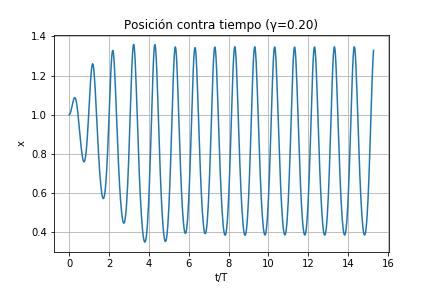
\includegraphics[height=5cm]{P1.png} \hspace*{\fill}
    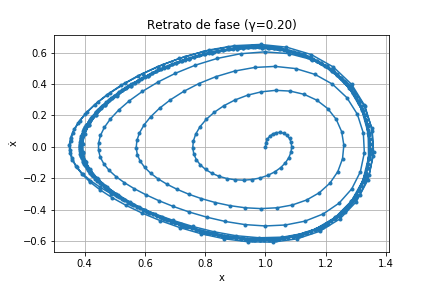
\includegraphics[height=5cm]{R1.png}
\end{center}

\begin{center}
	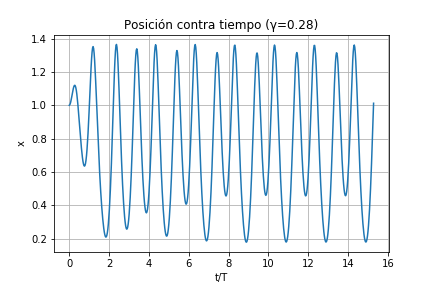
\includegraphics[height=5cm]{P2.png} \hspace*{\fill}
    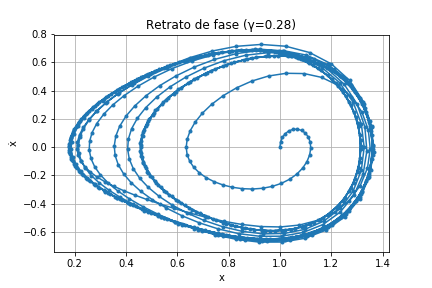
\includegraphics[height=5cm]{R2.png}
\end{center}

\begin{center}
	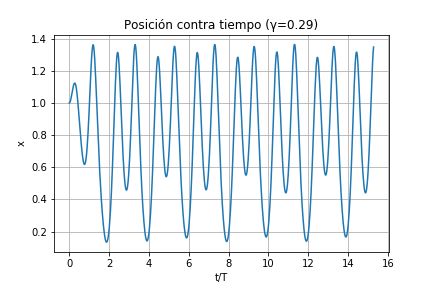
\includegraphics[height=5cm]{P3.png} \hspace*{\fill}
    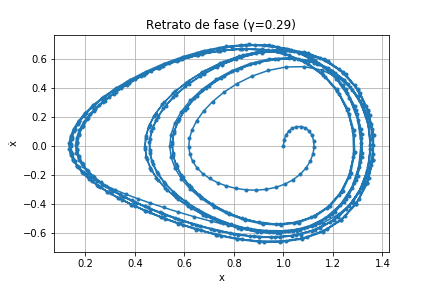
\includegraphics[height=5cm]{R3.png}
\end{center}

\begin{center}
	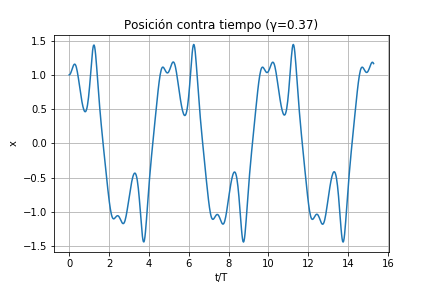
\includegraphics[height=5cm]{P4.png} \hspace*{\fill}
    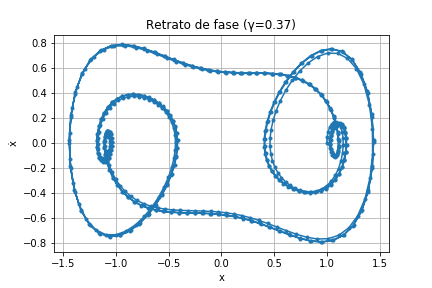
\includegraphics[height=5cm]{R4.png}
\end{center}

\begin{center}
	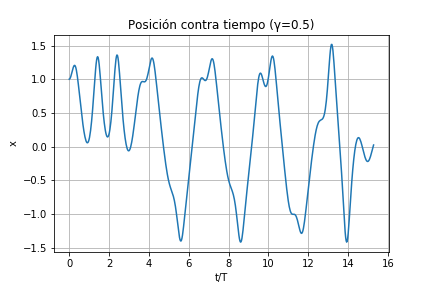
\includegraphics[height=5cm]{P5.png} \hspace*{\fill}
    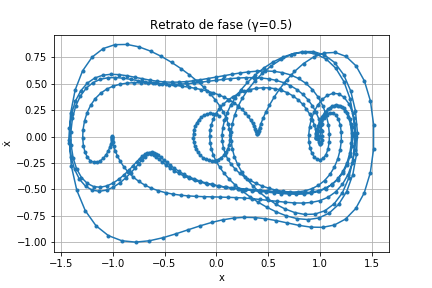
\includegraphics[height=5cm]{R5.png}
\end{center}

\begin{center}
	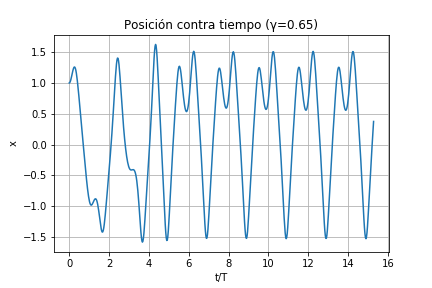
\includegraphics[height=5cm]{P6.png} \hspace*{\fill}
    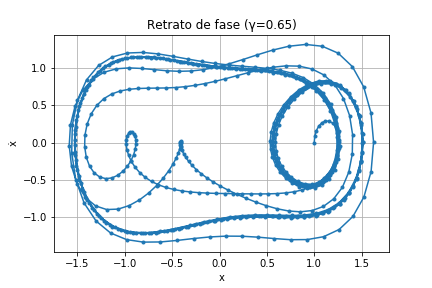
\includegraphics[height=5cm]{R6.png}
\end{center}

Aquí observamos que incrementando el valor de $\gamma$, que en la ecuación de Duffing representa el valor de la fuerza impulsora, obtenemos un comportamiento cada vez más distinto en las gráficas.


\section{Conclusiones}
En los diagramas de posición contra tiempo mostrados, así como retratos de fase, podemos observar cómo al variar ligeramente uno de los parámetros de la ecuación obtenemos comportamientos sumamente diferentes, especialmente si comparamos $\gamma=0.20$ con $\gamma=0.65$. Estos son ejemplos de comportamientos caóticos, mostrando que la ecuación de Duffing exhibe este tipo de conducta.

\section*{Bibliografía}
\begin{itemize}
\item \\Edward Lorenz. Recuperado el 27 de mayo de 2019 desde \\https://www.um.es/docencia/barzana/BIOGRAFIAS/Biografia-Edward-Lorenz.php
\\

\item \\Chaos theory. Recuperado el 27 de mayo de 2019 desde \\https://en.wikipedia.org/wiki/Chaos\_theory
\\

\item \\Efecto mariposa. Recuperado el 27 de mayo de 2019 desde \\https://es.wikipedia.org/wiki/Efecto\_mariposa
\\

\item \\Atractor de Lorenz. Recuperado el 27 de mayo de 2019 desde \\https://es.wikipedia.org/wiki/Atractor\_de\_Lorenz
\\

\item \\Teoría de las Bifurcaciones. Recuperado el 27 de mayo de 2019 desde \\http://www.dinamica-de-sistemas.com/cursos/syswa5x3.htm
\\




\end{itemize}
\end{document}
